\chapter{Introduction}
\label{chap:intro}

\section{Prelude}

Two of the most foundational observations of the Earth system are 
(1) that the planet is cooling off from a combination of primordial heat and the decay of radioactive elements,
and (2) that it is rotating.
The cooling of the planet results in convection in Earth's interior and its surface expression in plate tectonics,
and is thus responsible for a great deal of the geologic activity that we experience.
The rotation of the planet is a dominant factor in the fluid dynamics of the oceans, atmosphere, and core.
In this dissertation we consider the interaction between convection in Earth's mantle and the rotational dynamics of the planet.
We may relate the two processes through the classical angular momentum equation.
Conservation of angular momentum in a rotating reference frame for a torque free planet requires
\begin{equation}
\frac{\partial \mathbf{H}}{\partial t} + \mitbf{\Omega}\times\mathbf{H} = 0,
\label{eq:conserve_momentum_rotating}
\end{equation}
where the angular momentum $\mathbf{H}$ is given by $\mathbf{H} = \mathbf{I}\cdot\mitbf{\Omega}$,
$\mathbf{I}$ is the moment of inertia tensor, and $\mitbf{\Omega}$ is the angular velocity vector.
For geologic processes the effects of inertia are negligible, so the inertial
term $\partial \mathbf{H} / \partial t$ may be neglected, and the conservation equation becomes 
\begin{equation}
\mitbf{\Omega}\times \left(\mathbf{I} \cdot \mitbf{\Omega}\right)= 0.
\label{eq:constraint}
\end{equation}
Convection in Earth's mantle, by its very nature, involves the transfer mass of different densities,
as cold lithosphere sinks into the mantle, and buoyant plumes rise from the core mantle boundary (CMB).
This transfer of mass changes the density structure of the mantle, thereby changing the moment of inertia.
Equation~\eqref{eq:constraint} is a strong constraint on $\mitbf{\Omega}$: if the moment of inertia
is a function of time, then the spin axis must also be a function of time.
The change in direction of a planet's spin axis as a response to a changing moment of inertia is known as true polar wander (TPW).
In the following sections we give a brief account of the history of conceptions of TPW,
as well as an overview of the content of this dissertation.

\section{A short history of true polar wander}

Although true polar wander as it is understood today is a relatively recent concept,
concerns about the stability of Earth and its place in the univserse are quite old.
Aristotle advanced a conception of nature that relied heavily on order and symmetry.
This philosophy entered into the worldview of early Mediterranean cartographers, who, knowing that
they lived in the northern hemisphere, postulated that there must be a large
southern continent to preserve symmetry and balance in the world \citep{wilford2001mapmakers}.
This hypothetical southern continent became known as \emph{Terra Incognita Australis}, from which
we get the name ``Australia''.

\begin{figure*}
\centering
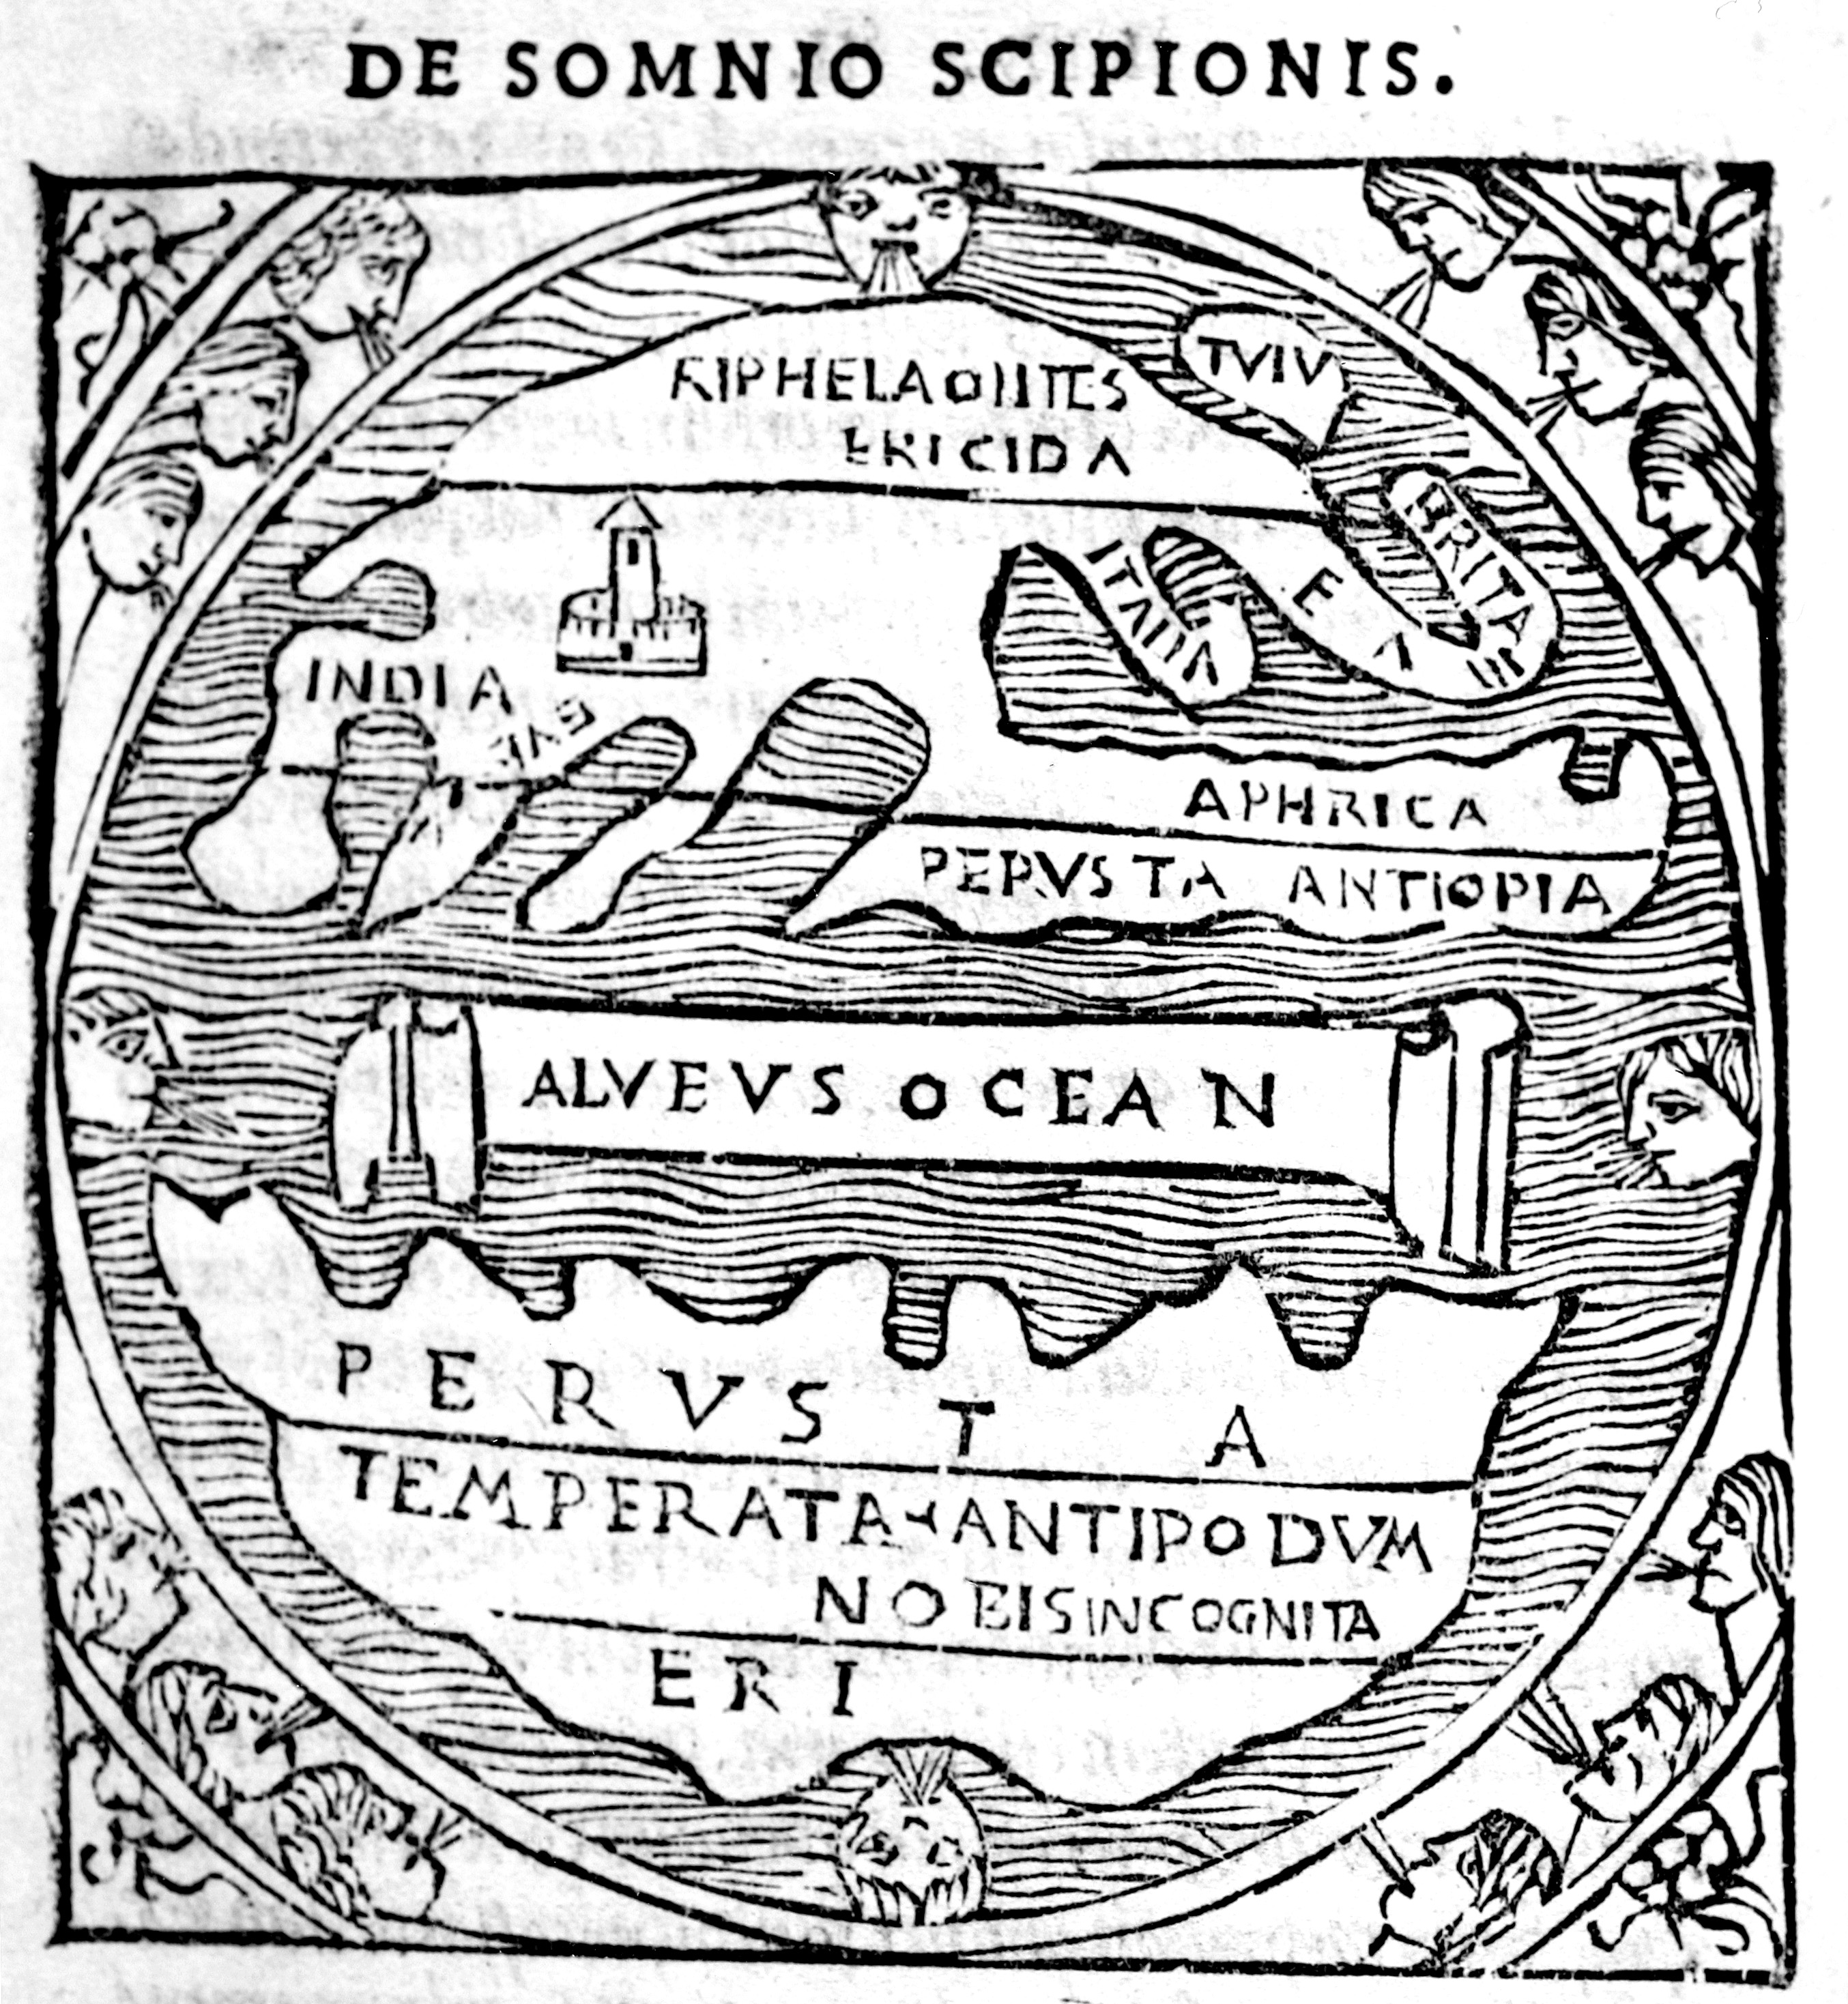
\includegraphics[width=0.5\textwidth]{intro/figures/macrobius.jpg}
\caption[Map of the world according to Macrobius.]{Map of the world according to Macrobius Ambrosius Theodosius in \emph{De Somnio Scipionis}, or \emph{Dream of Scipio}, \emph{ca.} 430 C.E..
It shows a great southern continent, which was thought to be very simliar to the known northern lands, and fed into the legend of \emph{Terra Australis}.
The map was reproduced and reinterpreted many times during the midieval period and Renaissance. This particular print comes from a 1515 reproduction.}
\label{fig:macrobius}
\end{figure*}

Among the earliest maps showing the southern continent was that of Macrobius Ambrosius Theodosius, a fifth
century Roman author. His map, from \emph{De Somnio Scipionis}, showed the large southern continent
largely mirroring the northern continents in shape and size (Figure~\ref{fig:macrobius}).
This map became hugely influential in midieval and Renaissance cartography \citep{stahl1942astronomy}.
During the Renaissance, ideas about Earth's place in the solar system famously became
entwined with Catholic theology. In the 17th century the Jesuit scholar Athanasius Kircher
published a series of treatises on geology and volcanology. In his \emph{Turris Babel} (1679)
Kircher interpreted the Biblical story of the Tower of Babel as meaning that 
the tower was intended to reach the moon. He performed a series of calculations
about how much material would be needed to build such a tower, determined where the planet's new
center of mass would be, and concluded:
``\ldots the motion of the earthly globe from it center would bring the total ruin of nature below'' (see Figure~\ref{fig:turris_babel}).

\begin{figure*}
\centering
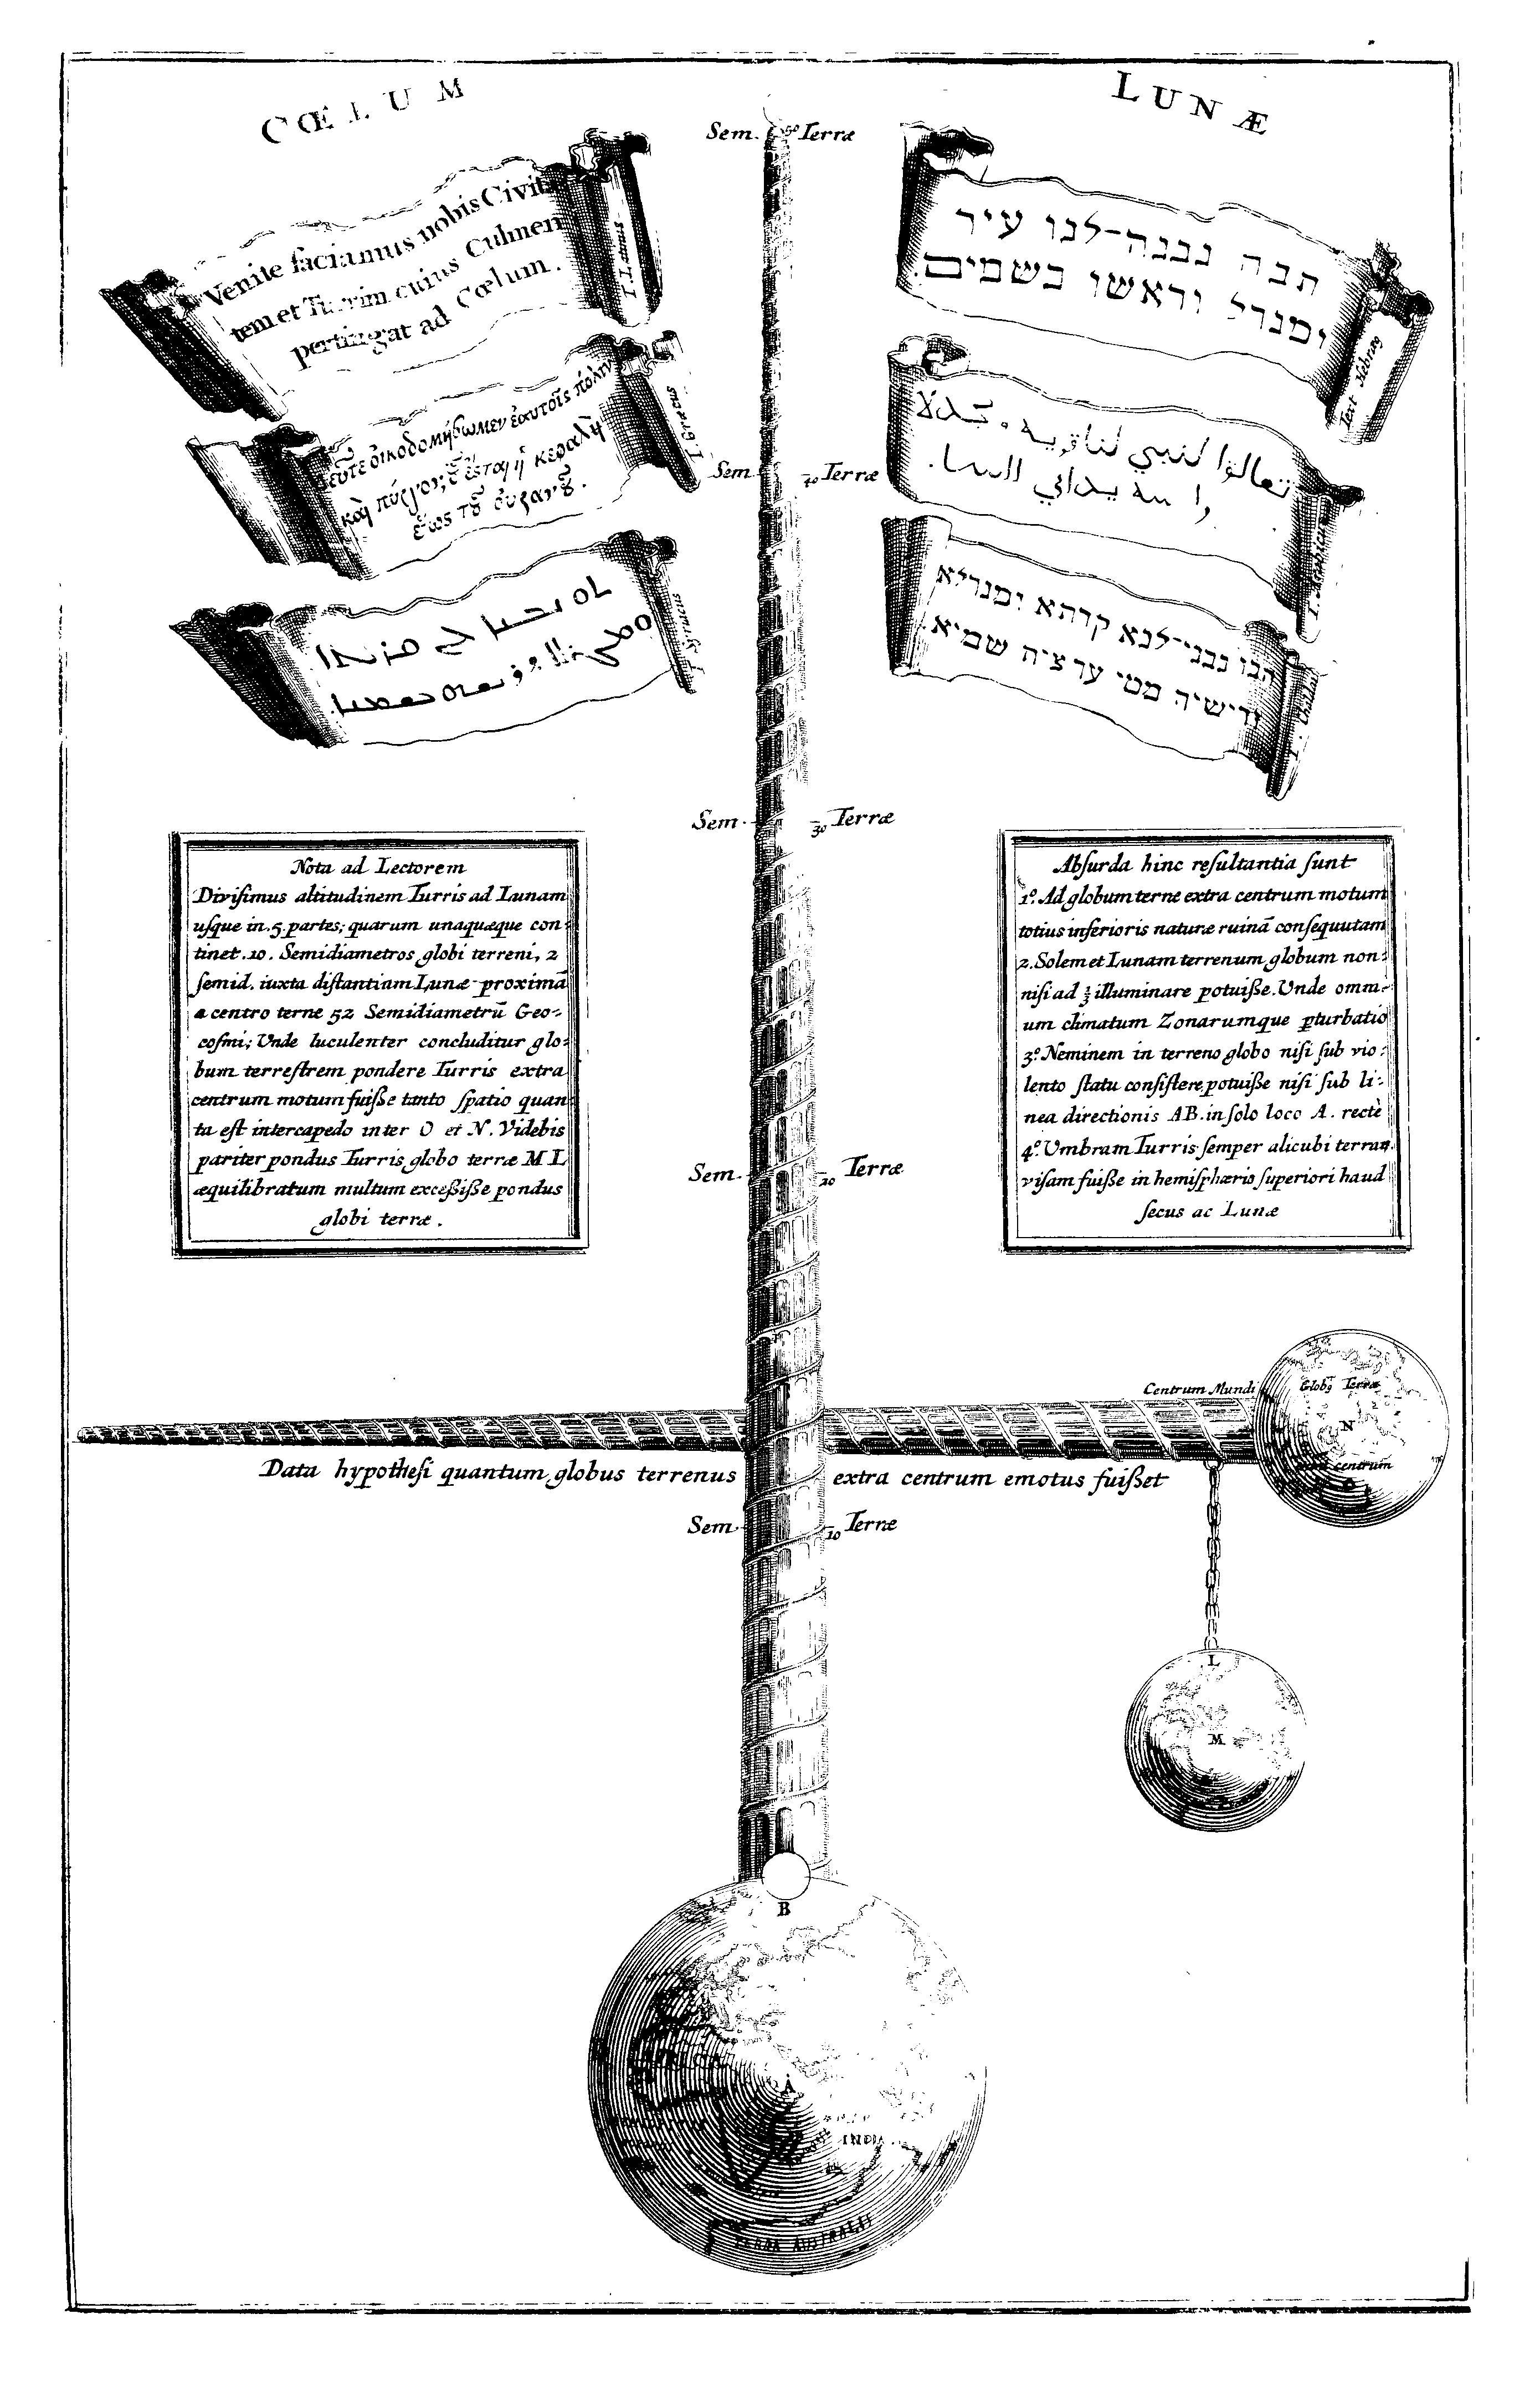
\includegraphics[width=0.75\textwidth]{intro/figures/turris_babel.jpg}
\caption[Plate from \emph{Turris Babel} (1679), by Athanasius Kircher.]{Plate from \emph{Turris Babel} (1679), by Athanasius Kircher.
A fanciful thought experiment about the consequences of building the Tower of Babel to the moon.}
\label{fig:turris_babel}
\end{figure*}

A more modern approach to Earth's stability can be found in Newton's \emph{Principia} (1687),
where he describes the tendency of mass anomalies to move towards the equator of a spinning object:
\begin{quote}
\ldots let there be added anywhere between the pole and the equator a heap of new matter like a mountain,
and this, by its continual endeavor to recede from the center of its motion, will disturb the motion of the globe, 
and cause its poles to wander about its surface describing circles about themselves and the points opposite them.
Neither can this enormous deviation of the poles be corrected otherwise than by placing that mountain either in
one of the poles\ldots or in the equatorial regions\ldots
\end{quote}

During the 18th and 19th centuries, as the science of geology developed, catastrophic polar wandering
became a possible explanation for the puzzling paleoclimatic and paleontologic findings, such as coal
seams in Svalbard and low-latitude glacial deposits \citep{barrell1914status}.
Alfred Wegener, most famous for origninating the theory of continental drift,
published a paleoclimatology book with Wladimir K\"oppen \citep{koppen1924} which,
in addition to providing a continental reconstruction, attempted infer a paleopole
position from their data.

The first scientist to approach polar wandering from a quantitative perspective was
George Darwin (son of Charles) in 1887. In a manuscript given before the Royal Society \citep{darwin1887influence}
he described what is essentially the modern concept of true polar wander:
\begin{quote}
\ldots If the earth were a viscous fluid there is no doubt that the pole of the figure would
tend to displace itself towards the instantaneous axis\ldots 
But Sir William Thomson has shown that the earth is sensibly rigid; 
and in any case the earth is not a viscous fluid, sensibly called, although it may be slightly plastic.
\end{quote}
In other words, he concluded that if Earth were sufficiently deformable, 
polar wandering would be inevitable, but he had been convinced by William Thompson (not yet Lord Kelvin)
that it was too rigid for large scale motion of the poles.

After Darwin there was little futher work on the physics of polar wandering
until the 1950s. At that time, the first geophysical evidence for polar wandering
was emerging in the form of paleomagnetism.
In a series of papers by Ken Creer, Keith Runcorn and Ted Irving 
\citep{creer1954direction, runcorn1955rock, creer1957geophysical} paleomagnetic data,
primarily from Britain and North America, showed that the north pole had apparently shifted significantly
since the Precambrian. They considered both continental drift and true polar wander
as possible explanations for this wandering, with a preference for polar wander due to its simplicity.
However, as more paleomagnetic evidence mounted \citep[e.g.][]{irving1958polar}, it became clear
that different continents displayed different paleomagnetic apparent polar wander paths,
and apparent polar wandering became more frequently ascribed to the new theory of plate tectonics.
This is also where the terminology of ``true polar wander'' begins, in order to distinguish
it from the apparent polar wander due to plate motions.

At the same time, the dynamical theory of true polar wander began to receive more attention,
as the geophysical evidence began mounting that, on geological timescales, Earth is more
plastic than rigid. \citet{gold1955instability} provided a qualitative description of
true polar wander that included the famous mixed-metaphor of a beetle crawling
around on a perfectly spherical Earth, the spin axis always trying to catch up with it,
``as with the ass and the carrot hanging from a stick held by the rider.''
Further important theoretical work came from \citet{munk1960rotation}.
\citet{goldreich1969some} pointed out that in a convecting system there
are many density anomalies contributing to the moment of inertia,
and they extended Gold's beetle thought experiment to include many beetles crawling over Earth's surface. 
In this case the principal axes of Earth's moment of inertia do not track any one beetle,
and they may move faster than the beetles crawl.

In more recent years there has been renewed interest in true polar wander as an important process in Earth history.
A rapid reorientation of the solid Earth would have enormous conequences for paleoclimate \citep{kirschvink1997evidence},
as the poles could become tropics, and the tropics poles. The readjustment of the rotational
bulge would cause global shifts in sea level \citep{mound1999sea}.
These effects could have had a profound impact on the history of life \citep[e.g][]{kirschvink2003methane}.
Furthermore, as we have explored the solar system it has become clear that TPW
may be an important process on other planetary bodies as well.
TPW has been suggested as an explanation for features on Mars \citep{perron2007evidence},
Enceladus \citep{nimmo2006diapir} and the Moon \citep{garrick2014tidal}.


\section{Overview}

Mass redistribution in a planet causes perturbations in its moment of inertia tensor,
which cause variations in that planet's spin axis. This mass redistribution can
arise from many sources, including mantle convection \citep{spada1992excitation}, 
glacial loading and unloading \citep{chen2013rapid}, and oceans and atmospheres \citep{munk1960rotation}.
This dissertation focuses on true polar wander due to mantle convection, which has the largest and longest-period effect.
We develop the theory of true polar wander through scaling analyses,
numerical modeling, and the development new techniques for paleomagnetic data analysis.

In Chapter~\ref{chap:tpw_rate} we consider the problem of TPW from the perspective of fluid dynamics.
We present scaling analyses and numerical simulations of TPW due to mantle convection over a range of parameter space relevant to planetary interiors. 
For simple rotating convection, the most important parameters are the Rayleigh number, the rotation rate, and the size of relative density fluctuations 
(i.e. thermal expansivity times the temperature variations). 
We identify timescales for the growth of moment of inertia perturbations due to convection and for their relaxation due to true polar wander. 
These timescales, as well as the relative sizes of convective anomalies, control the rate and magnitude of TPW.
This analysis also clarifies the nature of so called ``inertial interchange'' TPW events, and when they are likely to occur.
Finally, we discuss implications for large-scale TPW in Earth's past.

In Chapter~\ref{chap:free_surface} we describe the development of numerical methods
for geodynamic models with a free-surface boundary condition.
Geodynamic simulations increasingly rely on simulations with a true free surface to 
investigate questions of dynamic topography, tectonic deformation, and
global mantle convection. In particular, gravity and moment of inertia perturbations
due to internal mantle density anomalies (crucial for TPW analyses) are modified by the deflections at a free surface.
However, implementations of free surface boundary conditions 
have proven challenging from a standpoint of accuracy, robustness, and stability.
In particular, time integration of a free surface tends to suffer from a numerical instability
that manifests as sloshing surface motions, also known as the ``drunken sailor'' instability.
This instability severely limits stable timestep sizes to those much smaller than could be used
in geodynamic simulations without a free surface. 
Several schemes have been proposed in the literature to deal with these instabilities.

We analyze the problem of creeping viscous flow with a free surface and discuss the 
origin of these instabilities. We demonstrate their cause and how existing stabilization 
schemes work to damp them out.
We also propose a new scheme for removing instabilities from free surface calculations. 
It does not require modifications to the system matrix, nor additional variables, but is instead
an explicit scheme based on nonstandard finite differences.  It relies on a single 
stabilization parameter which may be identified with the smallest relaxation timescale of the
free surface.

We also discuss the implementation of a free surface in the open source, community based
mantle convection software \texttt{ASPECT}.

In Chapter~\ref{chap:bayesian_plate_reconstruction} we develop a new Bayesian statistical approach
for analyzing paleomagnetic data.
Apparent polar wander (APW) paths from paleomagnetic poles provide the most direct data
for reconstructing past paleogeography and plate motions for times earlier than $\sim$200 Ma. 
Many of the proposed TPW events are derived from paleomagnetic APW paths.
However, it has proven difficult to interpret APW paths in the presence of large errors,
age uncertainties, and the lack of paleolongitude control in traditional paleomagnetic analysis.
Approaches for dealing with the uncertainties in APW paths include spline fits and running means.
We propose a new approach for interpretation of APW paths.
It extends the paleomagnetic Euler pole analysis of \citet{gordon1984paleomagnetic}
by placing it within the framework of a Bayesian inverse problem.
This allows the natural incorporation of uncertainties in both pole position and age.
The resulting paleomagnetic Euler poles provide estimates for the total
plate motions (not just the latitudinal components) as well as their uncertainties.

We show several example inversions on synthetic data to demonstrate the capabilities of the method.
We also show examples using real paleomagnetic data from Australia and 
from the Laurentian Keweenawan province. The latter inversion gives 
extremely rapid plate speeds, and we discuss the potential for TPW as an explanation.

\nocite{newton1728principia}
